% ============================ EXPERIMENTS ============================
\subsection{Platform and onboard pipeline}
We evaluate the flipper controllers both in simulation and on the real platform. The onboard perception pipeline that the map-based baselines
consume is representative of current practice: an Ouster LiDAR and IMU feed point-cloud
deskewing and LiDAR-ICP odometry~\cite{norlabicpmapper,libpointmatcher}, which drive elevation
mapping~\cite{fankhauser2018} to produce a robot-centric
elevation map, which we call the \emph{onboard map}.

\paragraph{Simulation comparison} We simulate in Gazebo~\cite{gazebo2004}, the simulator selected
for the virtual track of the DARPA Subterranean Challenge~\cite{roucek2022subt}. Unlike
typical simulators that approximate tracks with multiple wheels, we employ the track
simulation of~\cite{pecka2017tracks}, which models conveyor-belt behavior. The sensors match the real payload: a simulated Ouster OS0
($1024\times64$ rays at \SI{10}{\hertz}, \SIrange{0.1}{50}{\metre}, \SI{1}{\centi\metre}
Gaussian range noise) and a \SI{50}{\hertz} IMU with Gaussian noise and a slowly varying
bias. The simulation runs the same ROS~2 nodes as the real robot, so the onboard-map condition
runs the same ICP and elevation-mapping stack on these noisy streams; the ground-truth condition reads pose and map from the
simulator. The arena is the twelve-obstacle warehouse course of~\cite{cihala2025}
(Fig.~\ref{fig:obstacles}): a straight aisle lined with twelve numbered obstacles of
variable difficulty, including pallets, stacked boxes, planks, and a staircase.

\paragraph{Real robot comparison} The real arena repeats the protocol on one pallet obstacle between
two reset zones (Fig.~\ref{fig:robot}). AprilTag markers on the robot and in the arena,
seen by a camera on a stand, give an absolute localization that registers the handcrafted
ground-truth map.

\paragraph{Automated ride and \SAS{} override} In all reported runs the robot is
driven autonomously. A ride node drives the robot at a constant
\SI{0.6}{\metre\per\second} in simulation and, for safety, \SI{0.25}{\metre\per\second}
on the real robot. A controller that stalls inside a field is released
by the \emph{\SAS{} override}, which hands the flippers to \SAS{} until the robot moves
again, and the field is finished. A field not left
within \SI{120}{\second} is scored as not traversed.

\subsection{Baselines}
We compare against, in increasing autonomy: (i) \textbf{Manual control}, an expert
operator driving all four flippers by hand (the traversal-quality
ceiling~\cite{cihala2025}), and \textbf{Manual modes}, the operator switching between
preset flipper modes by hand~\cite{azayev2022}; (ii) the \textbf{\GC/\OA{}
controller}~\cite{cihala2025} in its automated form, where instead of the operator a
\SI{2}{\second} stuck timer switches the front flippers between \OA{} and \GC{}; (iii) every map-based controller catalogued in
Table~\ref{tab:sensing}; and our \textbf{\SAS}. Where the authors released code we run their
implementation; where they did not, we use our reimplementation from the paper, adapted
to a four-track robot. The geometry-based controllers were
adapted to the four-track morphology as follows. Chen's GFMP~\cite{chen2023} keeps the
exact two-contact solver and waypoint DP, but admits only flipper-supported contact cases,
since the chassis is passive, adds an absolute-pitch levelness cost, and uses the
four-track geometry and elevation-map profile. Yuan's configuration-space
planner~\cite{yuan2019} was reimplemented for the four-track link geometry, estimating step distance and height per tick from the onboard elevation
map instead of motion capture, replanning closed-loop and holding where the model is
undefined. Oehler and von Stryk's pose predictor~\cite{oehler2024}, given a four-flipper model
with a passive belly, gains the selection stage it lacks: a
43-candidate sweep commanding the highest-stability-margin configuration, holding when
no configuration is stable. Xu's HTO~\cite{xu2024} assumes a driven belly that carries the step edge;
with a passive belly the belly-contact regimes of its hybrid model are replaced on ascents by a
double-prop flipper bridge with enforced belly clearance, plus rear-release and
descent-preparation schedules. Zhang's planner~\cite{zhang2025} is reproduced only as its
contact-model pose prediction and action cost, solved at a virtual station
\SI{0.5}{\metre} ahead; chassis-supported poses are
forbidden on the passive belly.

\begin{figure*}[t]
  \centering
  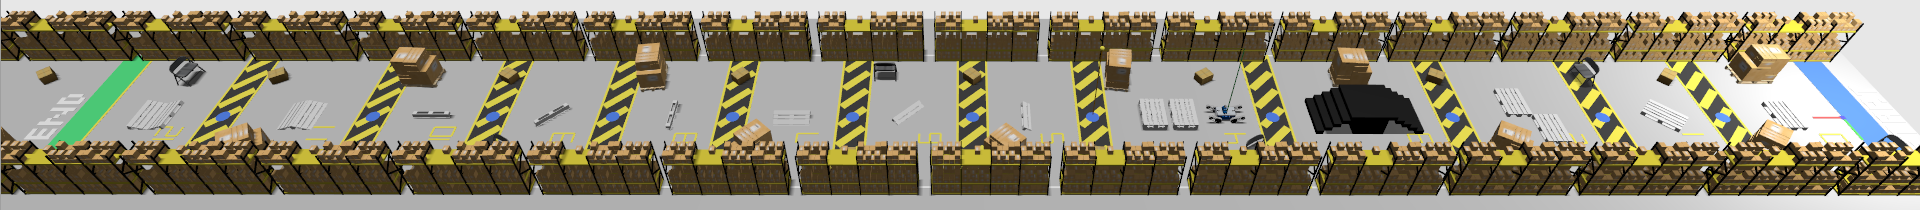
\includegraphics[width=\textwidth]{figures/gazebo_arena}
  \caption{\textbf{Automated simulation arena.} The Gazebo warehouse course
  of~\cite{cihala2025}: a straight aisle of twelve numbered obstacles of variable
  difficulty, each probing a different controller capability (pallets, stacked
  boxes, planks, and a staircase); the robot starts at the right. In the automated
  ride (Sec.~\ref{sec:experiments}) it is driven at a constant
  \SI{0.6}{\metre\per\second} through every field in turn, with a \SI{1}{\metre}
  settling strip between fields and a \SI{120}{\second} timeout per field.}
  \label{fig:obstacles}
\end{figure*}

\subsection{Ground-truth map for a fair baseline}
Our claim is that the onboard map is the limiting input, so evaluating the map-based
baselines under that map alone would conflate the controller with its perception. We
therefore run each of them twice:
once with the onboard map, and once with a \emph{ground-truth} map
that removes odometry drift. The gap between a
baseline's two scores measures its sensitivity to onboard mapping.

\subsection{Metrics}
Following~\cite{cihala2025} we report \textbf{traversal quality} (TQ), the mean of three
normalized sub-metrics: (a) \emph{acceleration/shock} $s$ from the IMU, (b) body
\emph{tilt} (roll/pitch magnitude), and (c) \emph{ground clearance}. All three are
computed against ground truth: in simulation the reference pose and map are read directly
from the simulator; on the real robot they come from external localization and a
handcrafted elevation map of the obstacle. The clearance score penalizes the deviation of the chassis clearance from its flat-ground
value outside a dead-band, linearly up to belly contact and \SI{10}{\centi\metre} above.
Rewarding raw clearance would favor baselines that freeze their flippers and coast in a
high pose.
\label{sec:metrics-block}%
Each channel is reduced over a traversal by a \emph{distance-binned maximum}. We bin by distance because we compare quality across the
obstacle, while each controller takes a different time to traverse it: every \SI{0.25}{\metre} of obstacle forms one bin, the
worst normalized sample in each bin is taken, and the bins are averaged; a field not
traversed scores $\mathrm{TQ}{=}0$. The raw streams are not low-pass filtered: shock is
the acceleration magnitude $|a|$ from the IMU at \SI{21}{\hertz}, normalized by
$N(s,s_{\max}/2)$~\cite{cihala2025}, with $s_{\max}=\SI{57.5}{\metre\per\second\squared}$
on the real robot and $s_{\max}=\SI{197}{\metre\per\second\squared}$ in Gazebo; clearance is the
closest ground point of a $10\times8$ grid on \SI{5}{\centi\metre} spacing under the
chassis. The three channels measure different things: over the traversed Gazebo
obstacles their pairwise Spearman correlations are $0.26$ (shock--clearance), $0.28$
(shock--tilt) and $0.39$ (clearance--tilt), and over the real crossings $0.06$, $0.39$ and
$-0.03$.

\begin{table*}[t]
\centering
\caption{\textbf{Traversal quality in Gazebo and on the real pallet.} Gazebo: mean over ten runs
of the twelve-obstacle course. Real: one ride of ten crossings per controller and map, mean over
the crossings, a crossing not completed scoring zero. All channels are scored against ground
truth, with $s_{\max}$ \SI{197}{\metre\per\second\squared} in Gazebo and
\SI{57.5}{\metre\per\second\squared} on the real robot. $\Delta$: TQ change under the onboard
map. \emph{Overrides}: activations of the \SAS{} override, per twelve-obstacle course in Gazebo
(mean over runs) and per ten-crossing ride on the real robot. Manual rides are hand-driven.
Best TQ in bold, second best underlined.}
\label{tab:results}
\footnotesize
\setlength{\tabcolsep}{3pt}
\begin{tabular*}{\textwidth}{@{\extracolsep{\fill}}lcccccccc@{}}
\toprule
 & \multicolumn{4}{c}{Gazebo, twelve obstacles} & \multicolumn{4}{c}{Real pallet, one ride of ten crossings} \\
\cmidrule(lr){2-5}\cmidrule(l){6-9}
Controller & \shortstack{TQ $\uparrow$\\GT map} & \shortstack{TQ $\uparrow$\\onboard map} & $\Delta$ $\uparrow$ & \shortstack{Overrides $\downarrow$\\GT / onboard} & \shortstack{TQ $\uparrow$\\GT map} & \shortstack{TQ $\uparrow$\\onboard map} & $\Delta$ $\uparrow$ & \shortstack{Overrides $\downarrow$\\GT / onboard} \\
\midrule
\multicolumn{9}{@{}l}{\emph{Manual}} \\
Manual control~\cite{cihala2025} & -- & 0.867 & -- & -- & -- & 0.810 & -- & -- \\
Manual modes~\cite{azayev2022} & -- & 0.825 & -- & -- & -- & 0.810 & -- & -- \\
\midrule
\multicolumn{9}{@{}l}{\emph{Reactive and geometry-based}} \\
{\v C}\'ihala \GC/\OA~\cite{cihala2025} & 0.800 & 0.780 & $-0.020$ & 0.1 / 0.0 & 0.612 & 0.657 & $+0.045$ & 0 / 0 \\
Chen GFMP~\cite{chen2023} & \underline{0.807} & \underline{0.787} & $-0.021$ & 5.0 / 6.2 & 0.660 & 0.661 & $+0.001$ & 10 / 10 \\
Yuan~\cite{yuan2019} & 0.807 & 0.783 & $-0.024$ & 7.3 / 5.9 & \underline{0.710} & \textbf{0.721} & $+0.012$ & 4 / 3 \\
Oehler~\cite{oehler2024} & 0.801 & 0.774 & $-0.028$ & 6.9 / 5.1 & 0.591 & 0.651 & $+0.060$ & 9 / 4 \\
Xu HTO~\cite{xu2024} & 0.783 & 0.768 & $-0.014$ & 6.0 / 5.9 & 0.685 & 0.677 & $-0.008$ & 10 / 10 \\
Zhang~\cite{zhang2025} & 0.790 & 0.774 & $-0.016$ & 7.4 / 9.0 & 0.689 & 0.693 & $+0.004$ & 10 / 10 \\
\midrule
\multicolumn{9}{@{}l}{\emph{Hierarchical}} \\
Azayev~\cite{azayev2022} & 0.763 & 0.746 & $-0.017$ & 4.6 / 4.2 & 0.662 & 0.694 & $+0.032$ & 0 / 0 \\
\midrule
\multicolumn{9}{@{}l}{\emph{Reinforcement learning}} \\
Pecka~\cite{pecka2016} & 0.781 & 0.765 & $-0.016$ & 6.0 / 6.7 & 0.642 & 0.640 & $-0.003$ & 0 / 0 \\
AT-D3QN~\cite{pan2023atd3qn} & 0.784 & 0.768 & $-0.016$ & 6.7 / 7.6 & 0.642 & 0.644 & $+0.002$ & 9 / 1 \\
ICM-D3QN~\cite{pan2023icm} & 0.779 & 0.770 & $-0.009$ & 6.5 / 7.7 & 0.652 & 0.548 & $-0.104$ & 10 / 14 \\
Mitriakov~\cite{mitriakov2021} & 0.778 & 0.752 & $-0.026$ & 5.2 / 5.6 & \textbf{0.712} & 0.635 & $-0.077$ & 0 / 5 \\
C-TRAC~\cite{ctrac2025} & 0.789 & 0.680 & $-0.110$ & 0.0 / 16.0 & 0.457 & 0.478 & $+0.020$ & 18 / 17 \\
PPO~\cite{sarga2026thesis} & 0.780 & 0.768 & $-0.012$ & 7.7 / 8.5 & 0.647 & 0.647 & $0.000$ & 0 / 0 \\
\midrule
\textbf{\SAS{} (ours)} & \textbf{0.813} & \textbf{0.793} & $-0.020$ & -- & 0.680 & \underline{0.703} & $+0.023$ & -- \\
\bottomrule
\end{tabular*}
\end{table*}

\subsection{Results}
Table~\ref{tab:results} reports TQ per controller in Gazebo under the ground-truth and
the onboard map, and how often the \SAS{} override had to release each controller. Every controller, \SAS{} included, loses quality under the onboard map, by
$0.01$ to $0.03$ (C-TRAC by $0.11$); \SAS{}, which reads no map, loses $0.020$ through its
LiDAR-ICP odometry cue alone, and frees itself without the \SAS{} override, which releases
the map-based controllers 4 to 9 times per course under either map. C-TRAC degrades the most
under the onboard map, by $0.11$, and shows most clearly that the onboard map raises the need
for the override: never overridden under the ground-truth map, it is released 16 times per
course under the onboard map; Chen, Zhang, Pecka, AT-D3QN, ICM-D3QN and PPO also need more
releases under the onboard map, Yuan, Oehler and Azayev fewer.
Sampled over the body footprint (the chassis and \SI{1.5}{\metre} ahead, at
\SI{5}{\centi\metre}) every \SI{0.25}{\second}, the height difference between the onboard
and the ground-truth map has a median absolute value of \SI{0.9}{\centi\metre} and a median
per-snapshot RMSE of \SI{2.6}{\centi\metre}, with 4\% of the cells off by more than
\SI{10}{\centi\metre}.
The onboard map also reports its own uncertainty, and in Gazebo it grows over every
obstacle: the median bound width of the cells under the body rises from
\SI{2.4}{\centi\metre} at the reset to \SIrange{4.5}{4.9}{\centi\metre} after
\SI{8}{\second} on the obstacle, and its 90th percentile from \SI{3}{\centi\metre} to
\SIrange{17}{20}{\centi\metre}, the occluded cells the controllers regulate on. On the real
robot the mapper's per-cell variance shrinks with fusion, from \SI{1}{\centi\metre} to
\SI{3}{\milli\metre}, and does not reflect the map error. In one
C-TRAC run under the ground-truth map the robot tipped over on obstacle~7, the only
tip-over in either campaign; that obstacle is scored as not traversed.

On the real pallet (Table~\ref{tab:results}) the operator remains the reference: manual
control and manual modes both score $0.81$, above every controller. Among the
controllers, Yuan and \SAS{} lead under the onboard map at $0.70$--$0.72$, Mitriakov and Yuan
under the ground-truth map at $0.71$, and with one ride per condition the difference between
the two maps is within the spread over crossings for most of them. \SAS{} is never
overridden and completes every crossing; the map-based
controllers that stall are released by the \SAS{} override up to 18 times per ride (C-TRAC),
and C-TRAC and ICM-D3QN abort crossings under either map. The largest degradations under the onboard map are
ICM-D3QN ($-0.10$) and Mitriakov ($-0.08$). Unlike in Gazebo, the onboard map does not raise the
number of releases on the real robot for most controllers: AT-D3QN drops from 9 to 1 per ride
and Oehler from 9 to 4, Chen, Xu, Zhang and C-TRAC stay at their level, and only ICM-D3QN
(10 to 14) and Mitriakov (0 to 5) need more. The tilt channel, the target of
the stabilization term, is where \SAS{} leads: $0.86$ in Gazebo, level with Chen and ahead of
the rest ($0.75$--$0.85$), and on the real pallet its maximum tilt over the ride is
\ang{11.5}, against \ang{12} to \ang{26} for the other controllers and \ang{36} for C-TRAC.
